\documentclass[10pt]{beamer}
\usetheme{Malmoe}
\usepackage[utf8x]{inputenc}
\usepackage{ucs}
\usepackage[english,russian]{babel}
\usepackage[OT1]{fontenc}
\usepackage{amsmath}
\usepackage{amsfonts}
\usepackage{amssymb}
\usepackage{graphicx}

\author{Третьяк И.Д.\\ Научный руководитель: Лебедев C.А.}
\title[SBP-SAT методы на сетках с локальным сгущением]{SBP-SAT методы горизонтальной аппроксимации уравнений динамики атмосферы на сетках с локальным повышением разрешения}
\setbeamercovered{transparent}
\setbeamertemplate{navigation symbols}{} 
\logo{
\includegraphics[width=0.8cm]{./images/logo.png}

\includegraphics[width=0.8cm]{./images/MIET-logo.jpg}} 
\institute{Институт вычислительной математики им. Г.И. Марчука\\[1mm] Национальный исследовательский университет <<Московский инситут электронной техники>>} 
%\date{} 
\subject{} 

\defbeamertemplate*{footline}{shadow theme}
{%
\leavevmode%
\hbox{\begin{beamercolorbox}[wd=.5\paperwidth,ht=2.5ex,dp=1.125ex,leftskip=.3cm plus1fil,rightskip=.3cm]{author in head/foot}%
\usebeamerfont{author in head/foot}\insertframenumber\,/\,\inserttotalframenumber\hfill\insertshortauthor
\end{beamercolorbox}%
\begin{beamercolorbox}[wd=.5\paperwidth,ht=2.5ex,dp=1.125ex,leftskip=.3cm,rightskip=.3cm plus1fil]{title in head/foot}%
\usebeamerfont{title in head/foot}\insertshorttitle%
\end{beamercolorbox}}%
\vskip0pt%
}
\begin{document}

\begin{frame}
\titlepage
\end{frame}

\begin{frame}{Введение}

Модели общей циркуляции атмосферы:
\begin{enumerate}
\item[•] Динамическое ядро
\item[•] Параметризации процессов подсеточного масштаба
\end{enumerate}

Основной путь улучшения качества прогнозов $\rightarrow$ повышение разрешения расчетной сетки.

\end{frame}



\begin{frame}{Введение}

Пути повышения детализации прогноза состояния атмосферы

1. Глобальное повышение разрешения расчетной сетки

\begin{enumerate}
\item[+] Повышение эффективного разрешения
\item[--] Быстрый рост требуемых вычислительных ресурсов
\end{enumerate}

2. Локальное повышение разрешения расчетной сетки

\begin{enumerate}
\item[+] Экономия вычислительных ресурсов
\item[+] Повышение эффективного разрешения в области сгущения
\item[--] Численные ошибки на границах блоков
\end{enumerate}
\end{frame}



\begin{frame}{Уравнения мелкой воды}
\textbf{Уравнения мелкой воды в векторно-инвариантной форме:}
$$
\begin{cases}
\frac{\partial \textbf{v}}{\partial t} = -(\xi+f)\textbf{k} \times \textbf{v}-\nabla(gh+K)\\
\frac{\partial h}{\partial t} = -\nabla \cdot (\textbf{v}h)
\end{cases}
$$

$\textbf{v} - $ вектор горизонтальной скорости, $h$ - толщина слоя жидкости, $\textbf{k}$ - вертикальный единичный вектор, $\xi = \textbf{k} \cdot \nabla \times \textbf{v}$ - относительная завихренность, $f$ - параметр Кориолиса, $K=\textbf{v}\cdot \textbf{v} \slash 2$ - плотность кинетической энергии.

\end{frame}



\begin{frame}{Расчетная сетка}

\begin{figure}[h]
\centering
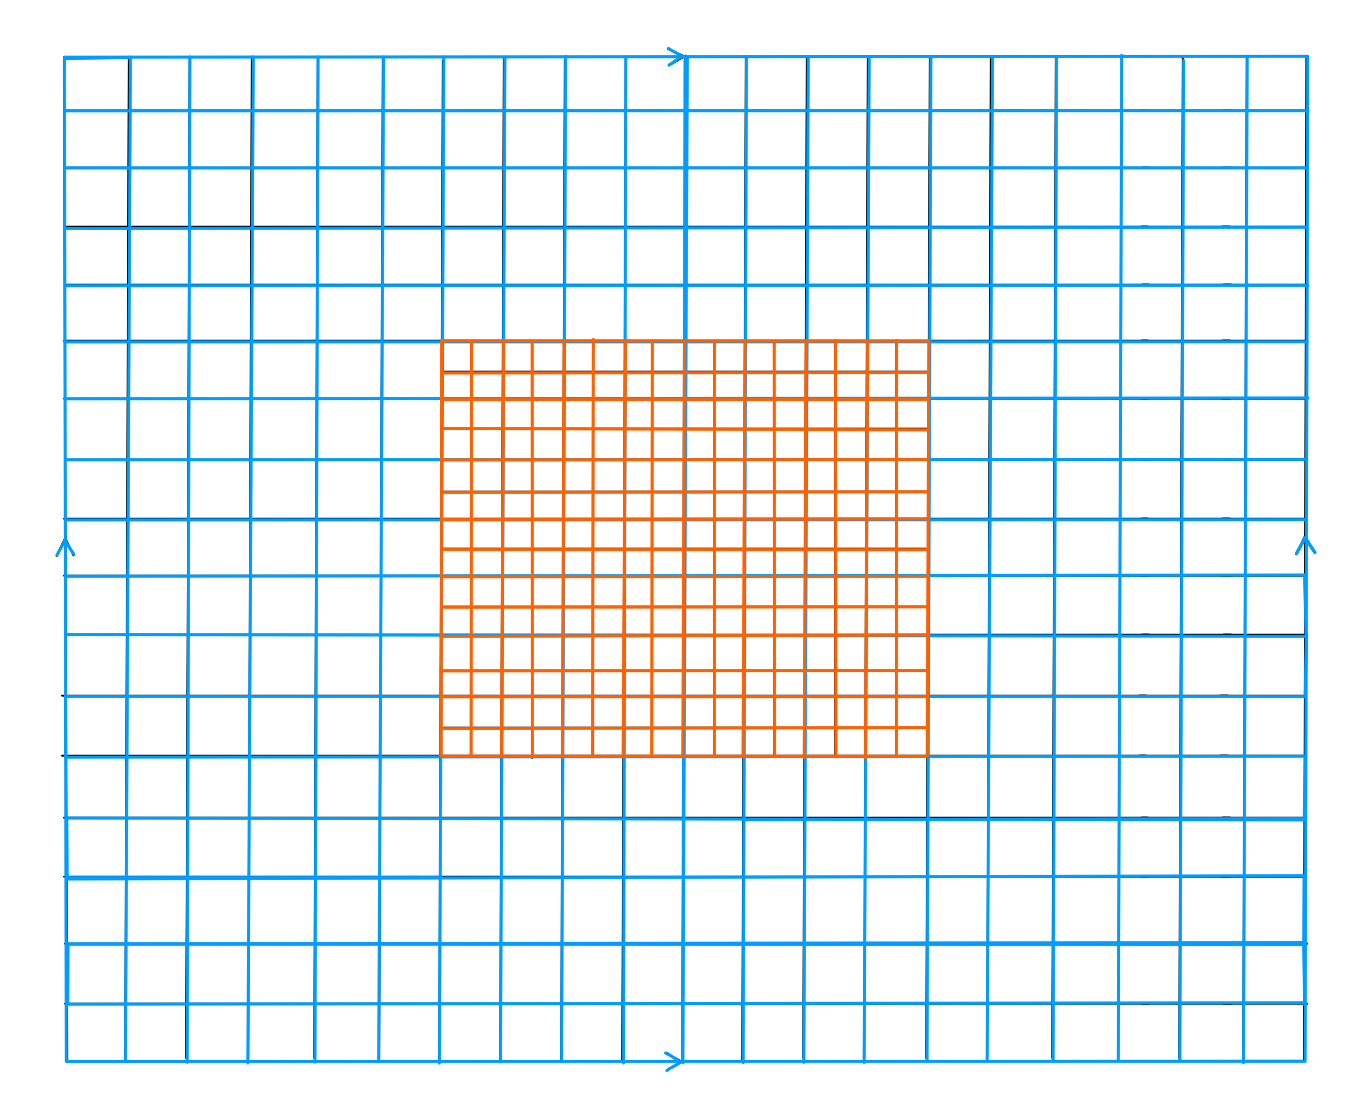
\includegraphics[width=0.8\linewidth]{./images/domain.png}
\caption{Возможная конфигурация расчетной сетки: бипериодические граничные условия, по середине блок с локальным уточнением в 2 раза.}
\label{fig:mpr}
\end{figure}

\end{frame}



\begin{frame}{Метод аппроксимации по пространству: Summation-by-parts finite differences}
$$\frac{\partial U}{\partial x}\approx D\textbf{u}$$

\textbf{Свойство суммирования-по-частям (Summation-by-parts или SBP):}
$$\textbf{u}^T HD \textbf{v} = (u_N v_N - u_0 v_0) -(D\textbf{u})^T H \textbf{v}$$

Дискретный аналог формулы интегрирования по частям:
$$\int\limits_{a}^bU(x)\frac{\partial V(x)}{\partial x}=U(b)V(b)-U(a)V(a)-\int\limits_{a}^b {V(x)\frac{\partial U(x)}{\partial x}}$$

\begin{enumerate}
 \item Выполнены дискретные аналоги законов сохранения массы и энергии.
 \item Теорема об устойчивости для линеаризованной задачи.
\end{enumerate}
\end{frame}



\begin{frame}{Формирование SBP-оператора}
$$D=H^{-1}Q$$
\begin{figure}[h]
\centering
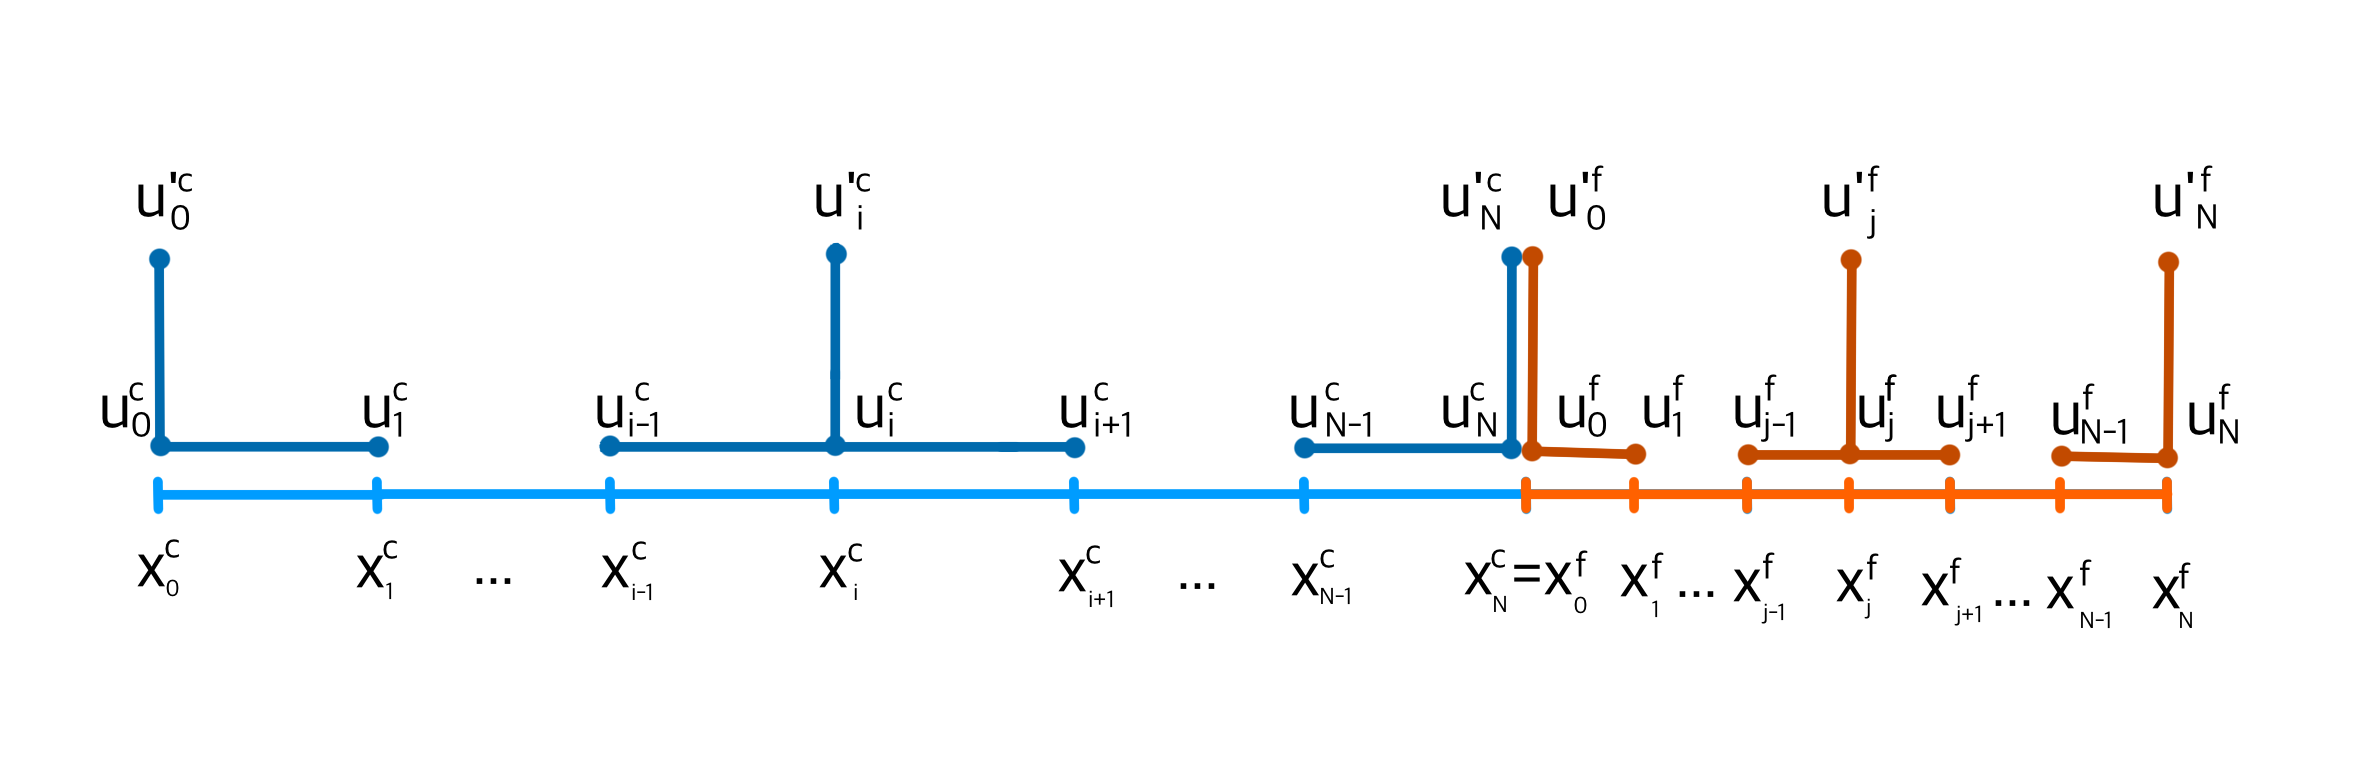
\includegraphics[width=0.9\linewidth]{./images/Q_scheme.png}
\caption{Шаблон разностной схемы для формирования матрицы Q}
\label{fig:mpr}
\end{figure}

Распространение на случай большей размерности:
$$\textbf{D}_x = D\otimes I, \ \textbf{D}_y = I \otimes D$$
$$\textbf{H}_x = H\otimes I, \ \textbf{H}_y = I \otimes H$$
\end{frame}




\begin{frame}{Условия на границах блоков: \\ (SAT) Simultaneous Approximation Terms}
\textbf{Формулировака условия неразрывности в слабой форме}
SAT-слагаемые:
$$\frac{\partial U}{\partial x}\approx D\textbf{u} + SAT_0 + SAT_N,$$

$$SAT_0=\sigma_0 (\Delta u^{left}), \ SAT_N=\sigma_N(\Delta u^{right})$$

Веса $\sigma_0, \sigma_N$ выбираются исходя из требования глобального сохранения энергии (выполнения SBP-свойства).

\begin{figure}[h]
\centering
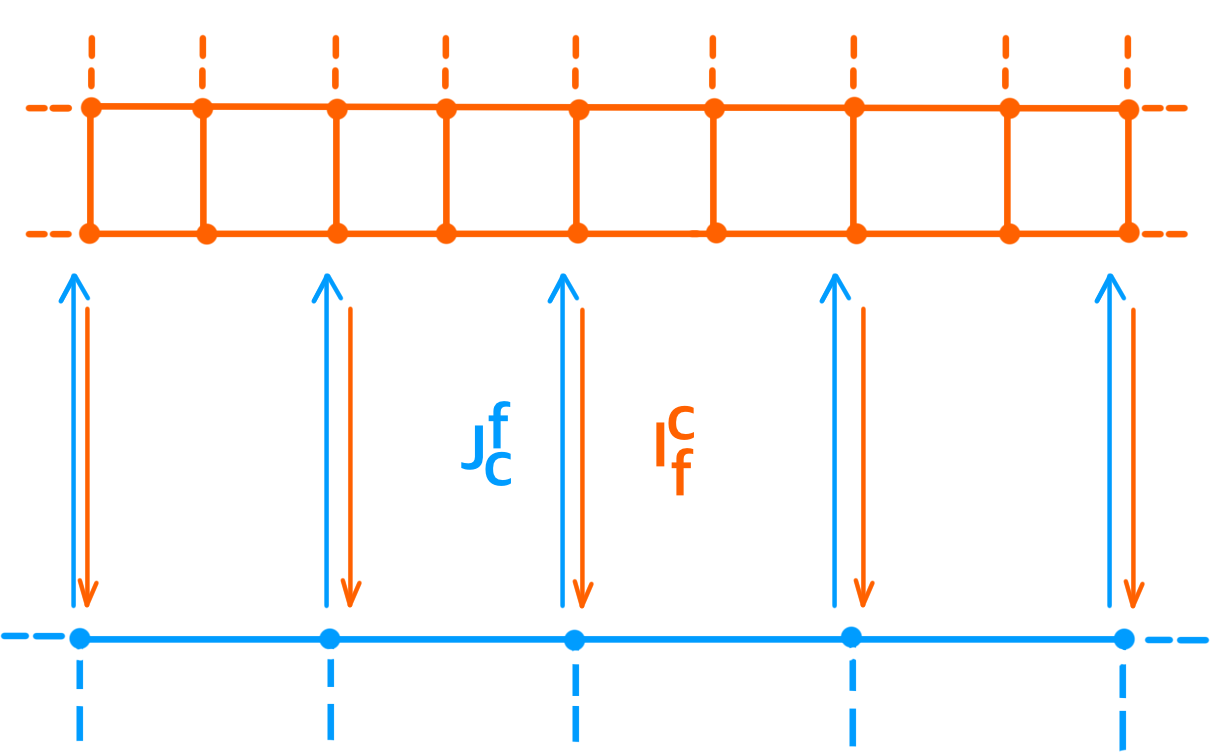
\includegraphics[width=0.5\linewidth]{./images/interp.png}
\caption{Интерполяция между блоками с различным разрешением}
\label{fig:mpr}
\end{figure}

\end{frame}




\begin{frame}{Неустойчивость Кельвина-Гельмгольца}

\begin{figure}[h]
\centering
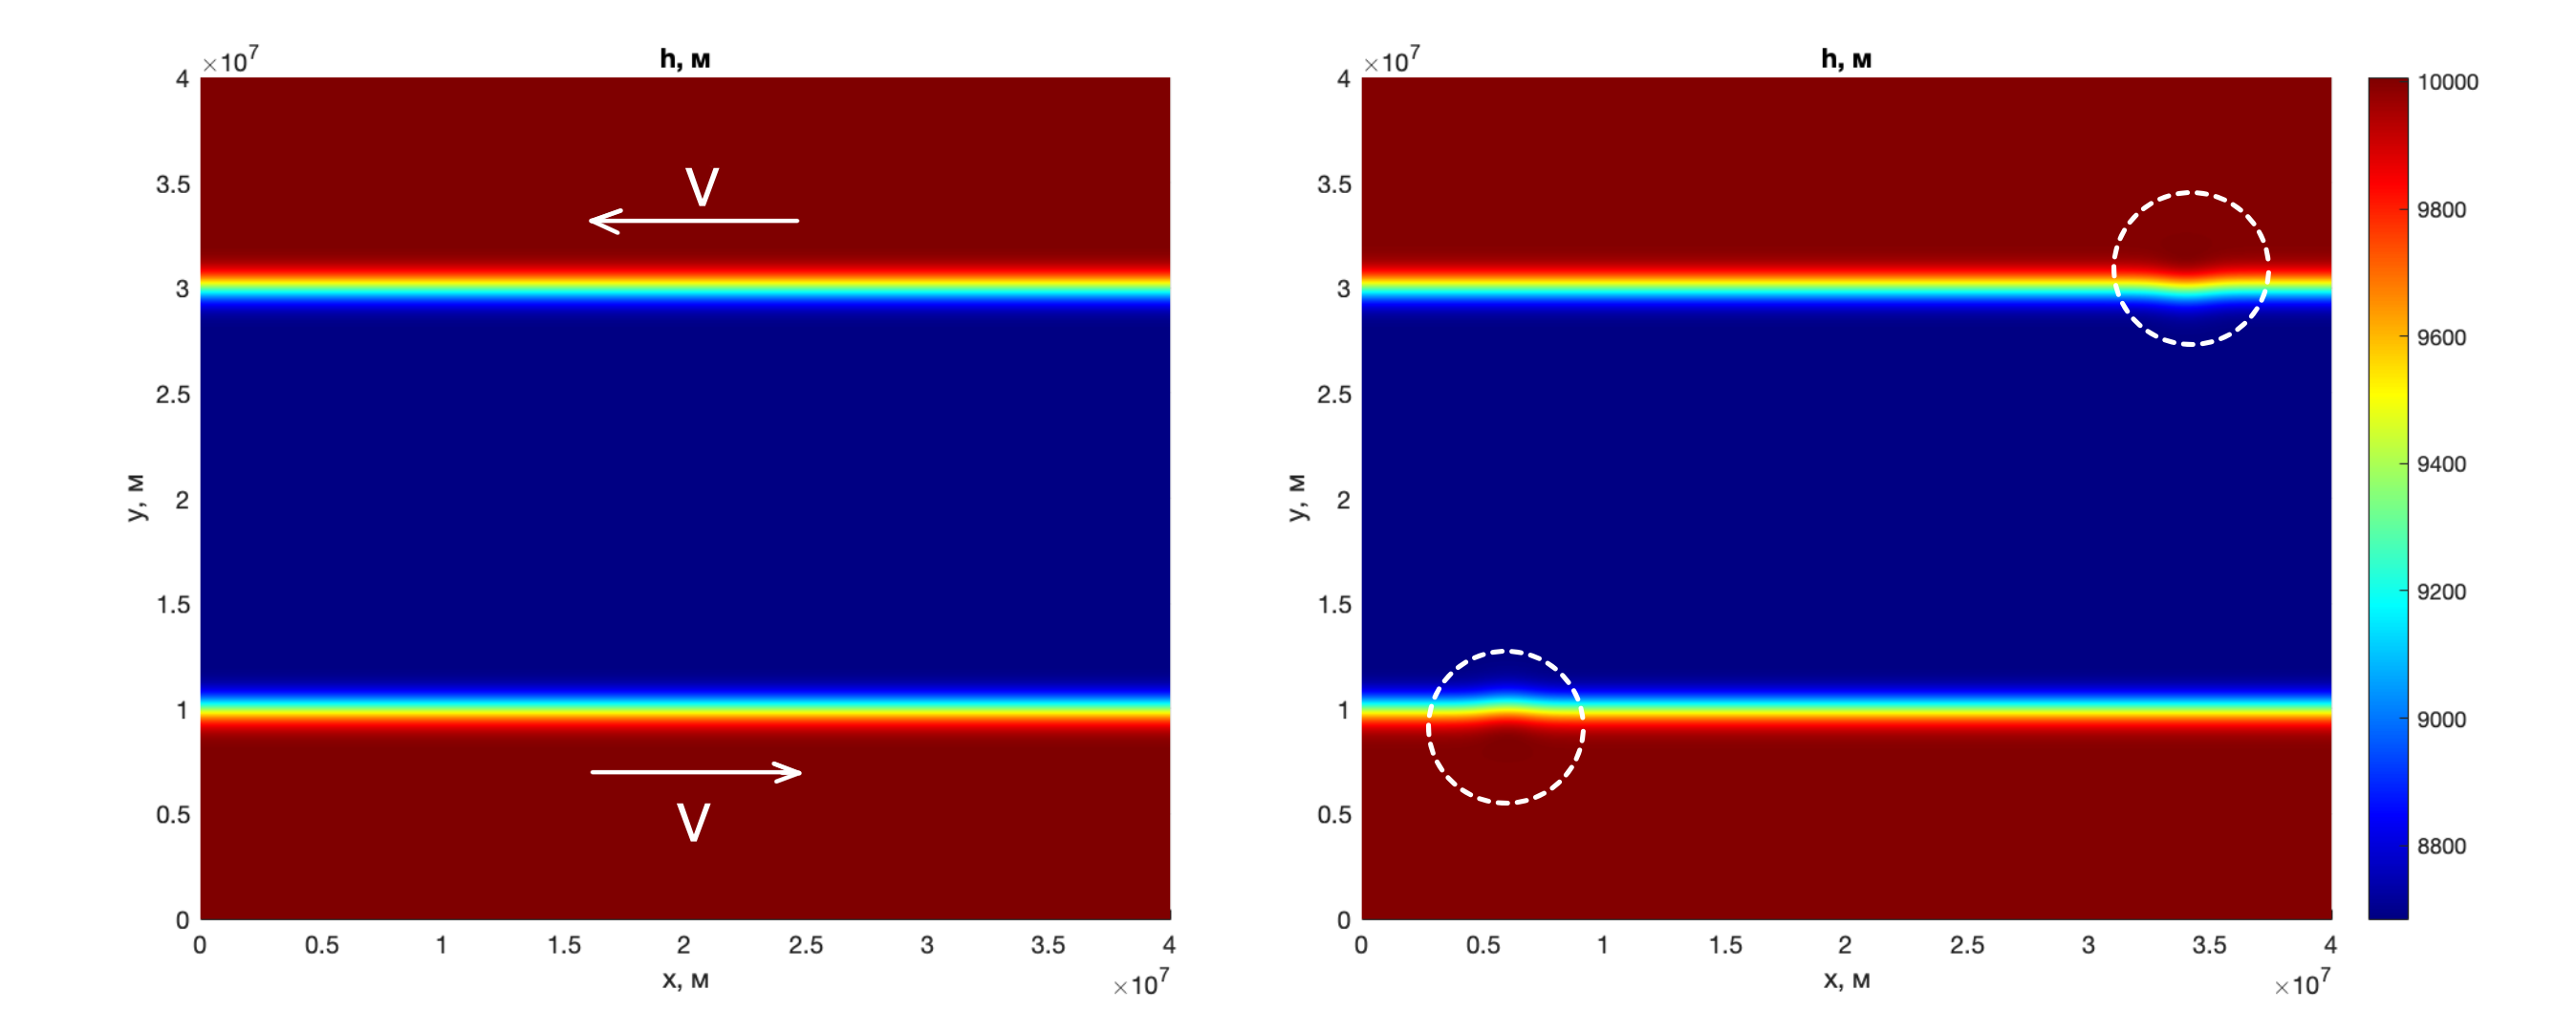
\includegraphics[width=1\linewidth]{./images/initial_cond_kelhelm.png}
\caption{Начальные условия для поля толщины слоя жидкости}
\label{fig:mpr}
\end{figure}

\end{frame}




\begin{frame}{Неустойчивость Кельвина-Гельмгольца}
\begin{figure}[h]
\centering
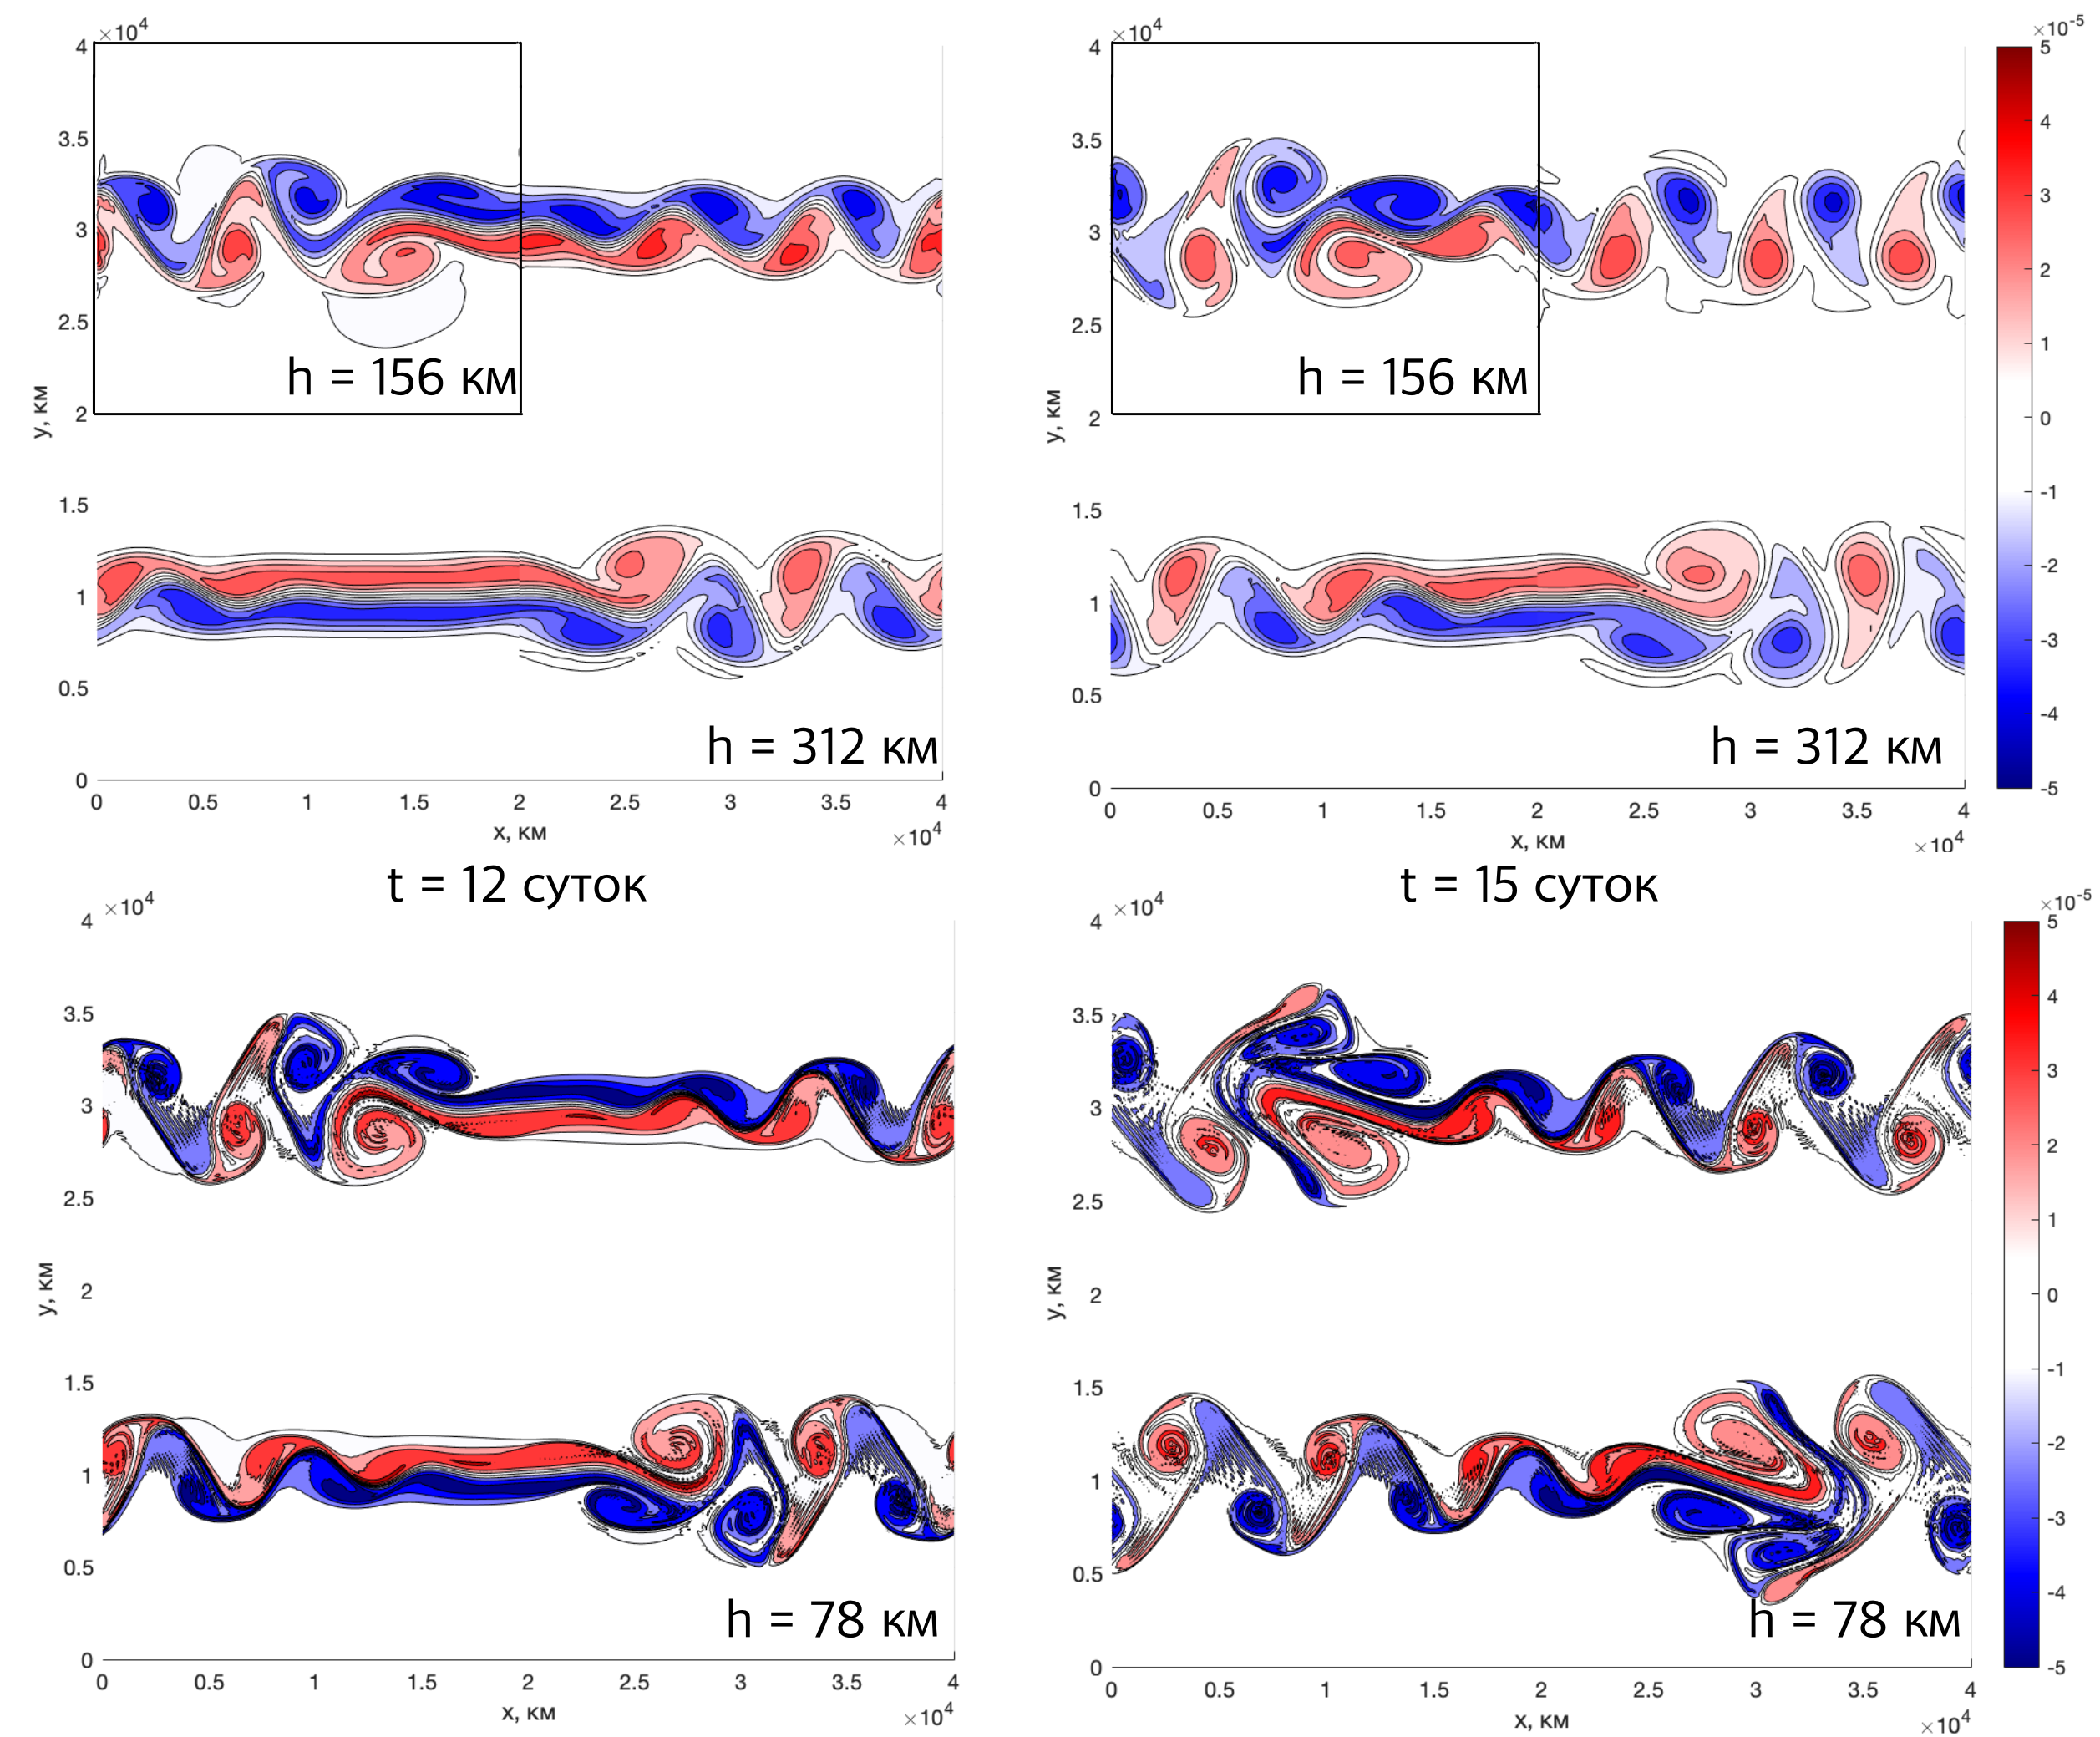
\includegraphics[width=0.8\linewidth]{./images/kelhelm_full.png}
\caption{Поле относительной завихренности (нижние рисунки - эталонное решение, верхние - решение с локальным сгущением) через 12 и 15 суток}
\label{fig:mpr}
\end{figure}
\end{frame}

\begin{frame}{Неустойчивость Кельвина-Гельмгольца}
\begin{figure}[h]
\centering
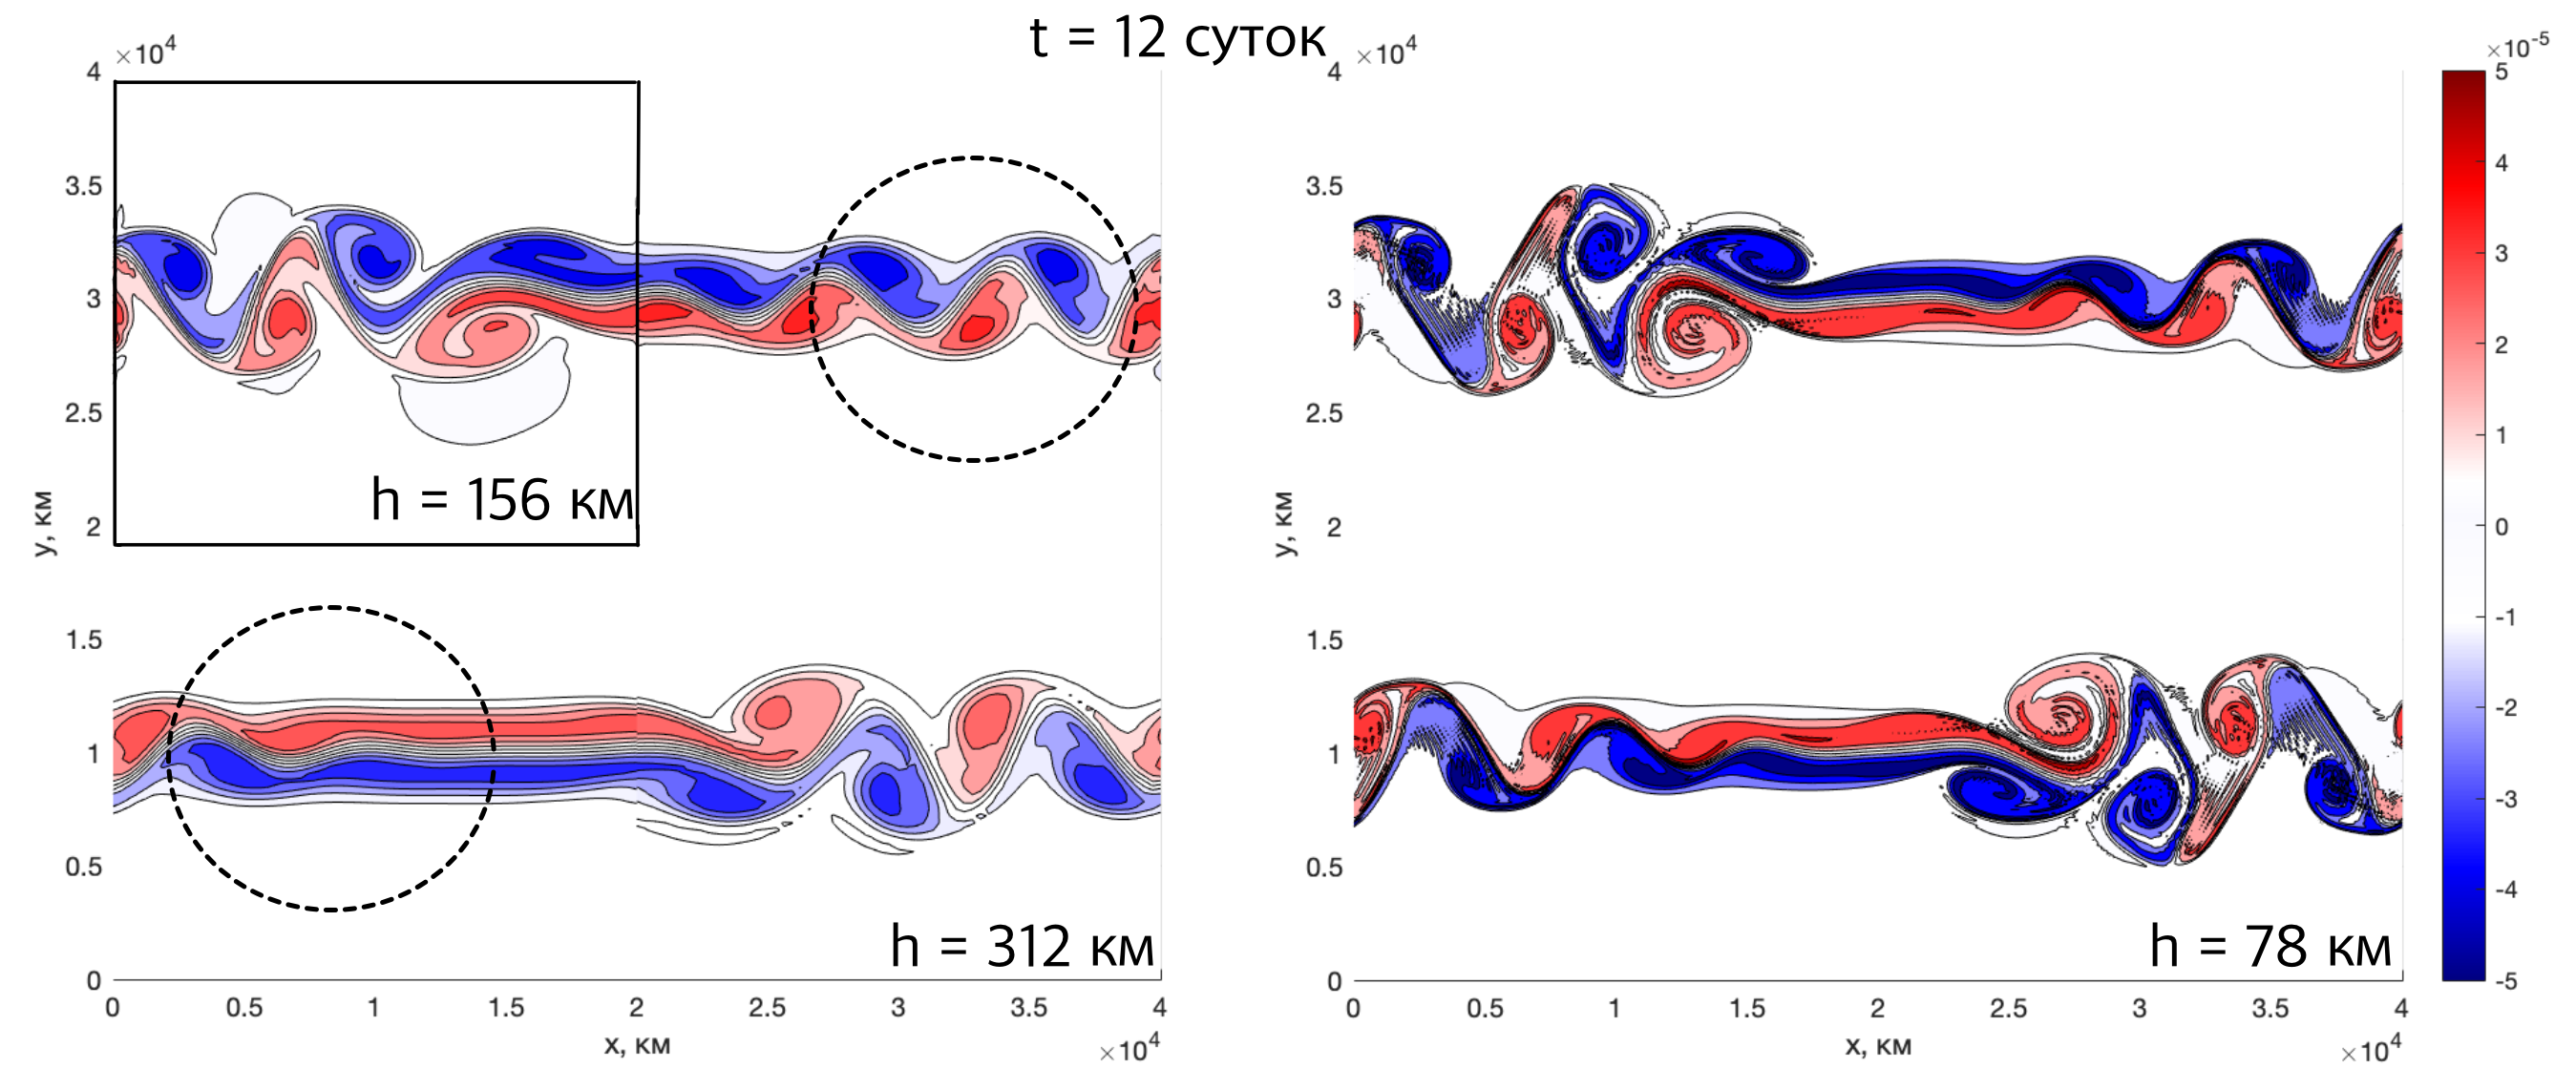
\includegraphics[width=1\linewidth]{./images/kelhelm12.png}
\caption{Поле относительной завихренности через 12 суток}
\label{fig:mpr}
\end{figure}
\end{frame}

\begin{frame}{Неустойчивость Кельвина-Гельмгольца}
\begin{figure}[h]
\centering
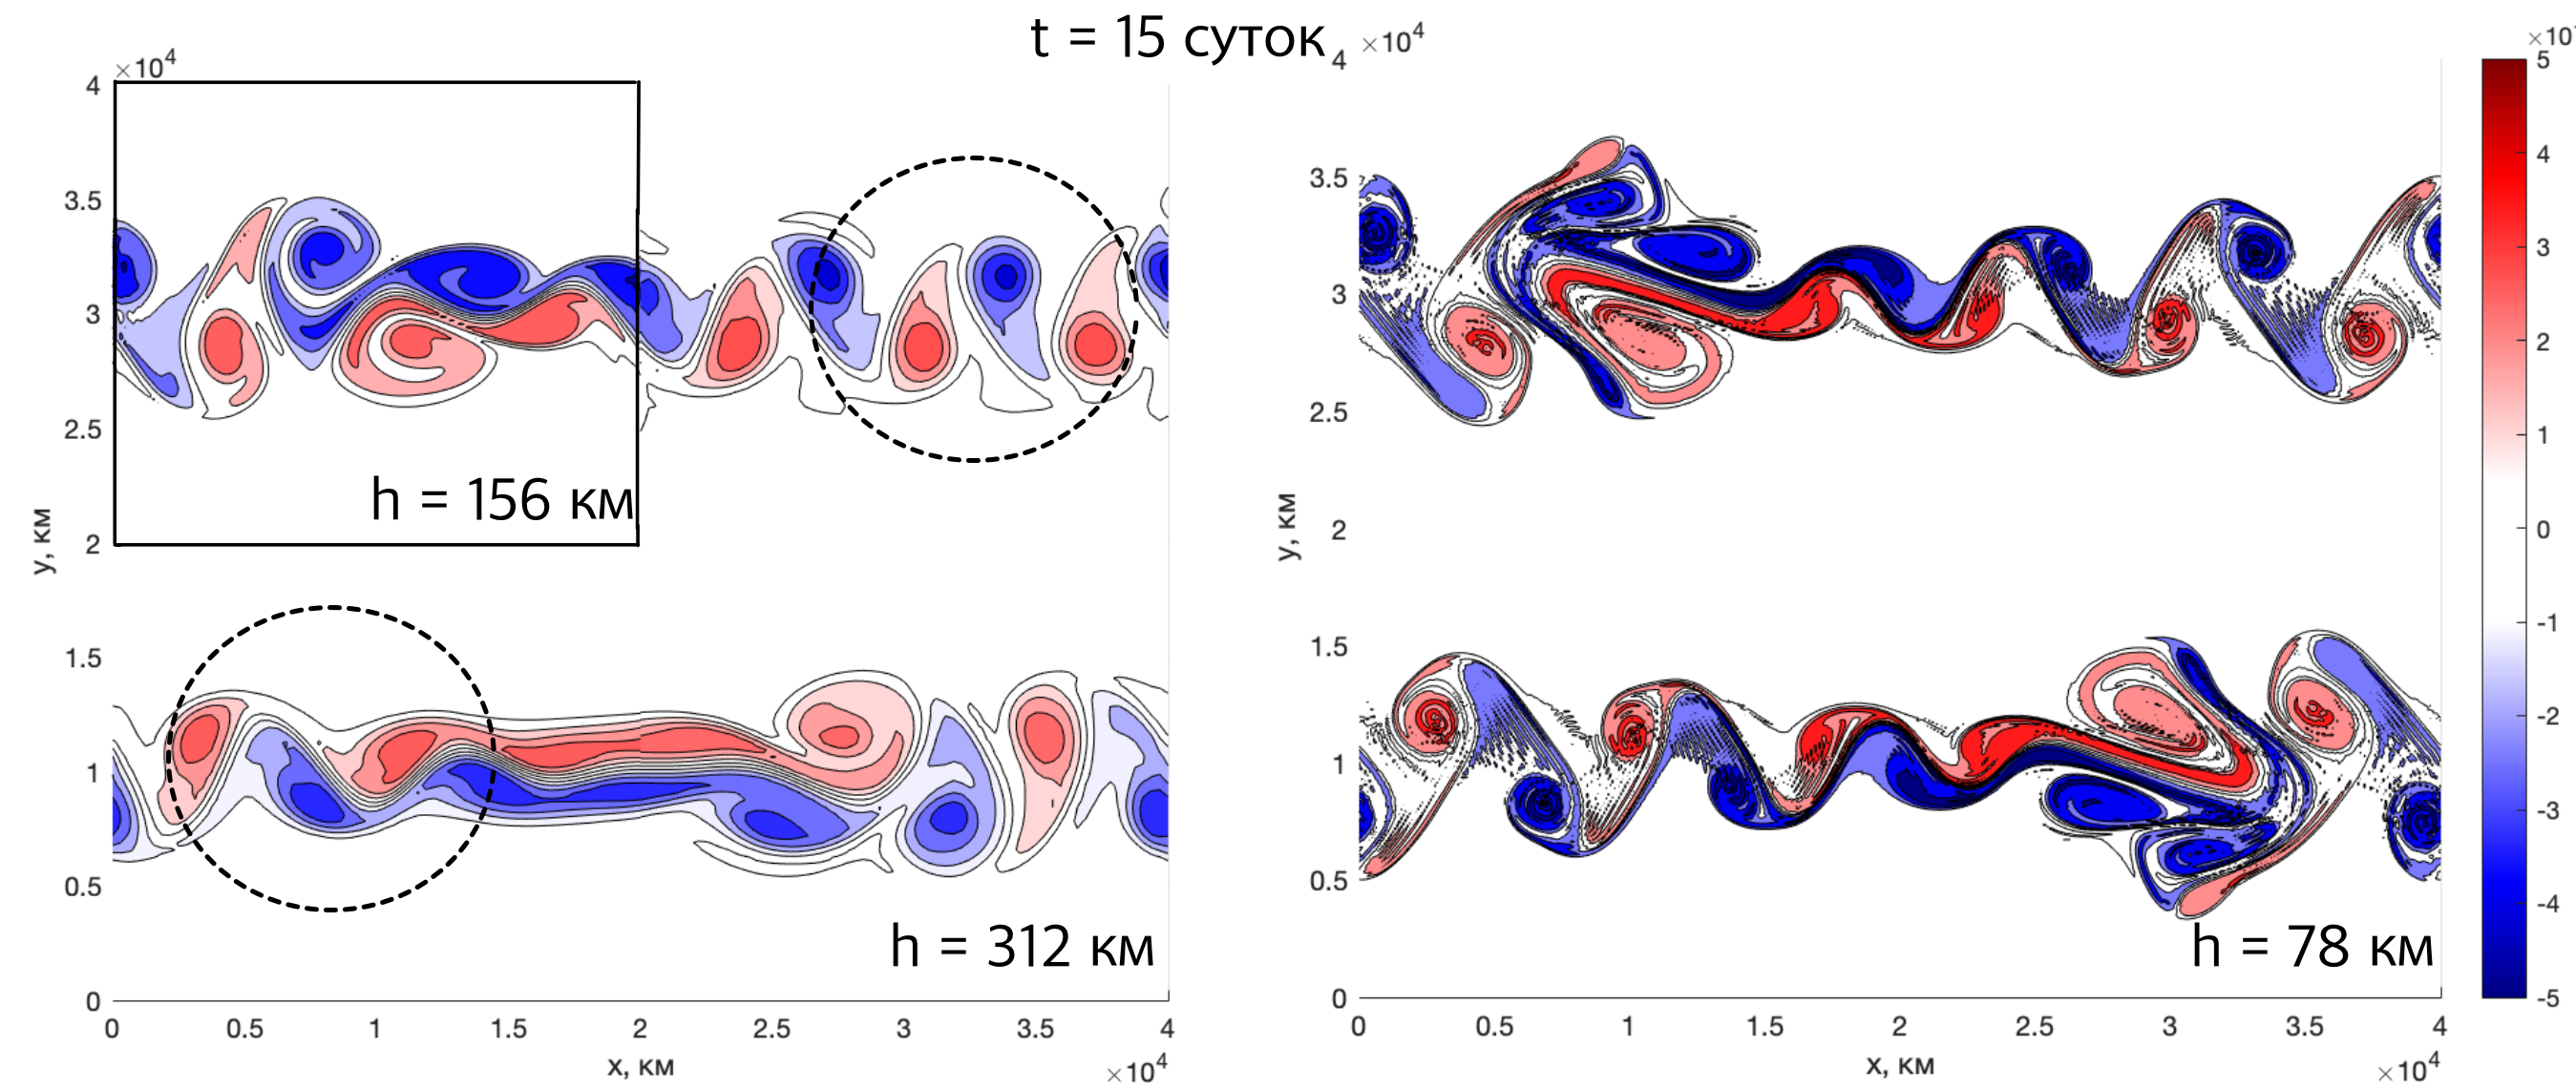
\includegraphics[width=1\linewidth]{./images/kelhelm15.png}
\caption{Поле относительной завихренности через 15 суток}
\label{fig:mpr}
\end{figure}
\end{frame}

\begin{frame}{Взаимодействующие тропические циклоны}

Поведение эталонного решения:
\begin{figure}[h]
\centering
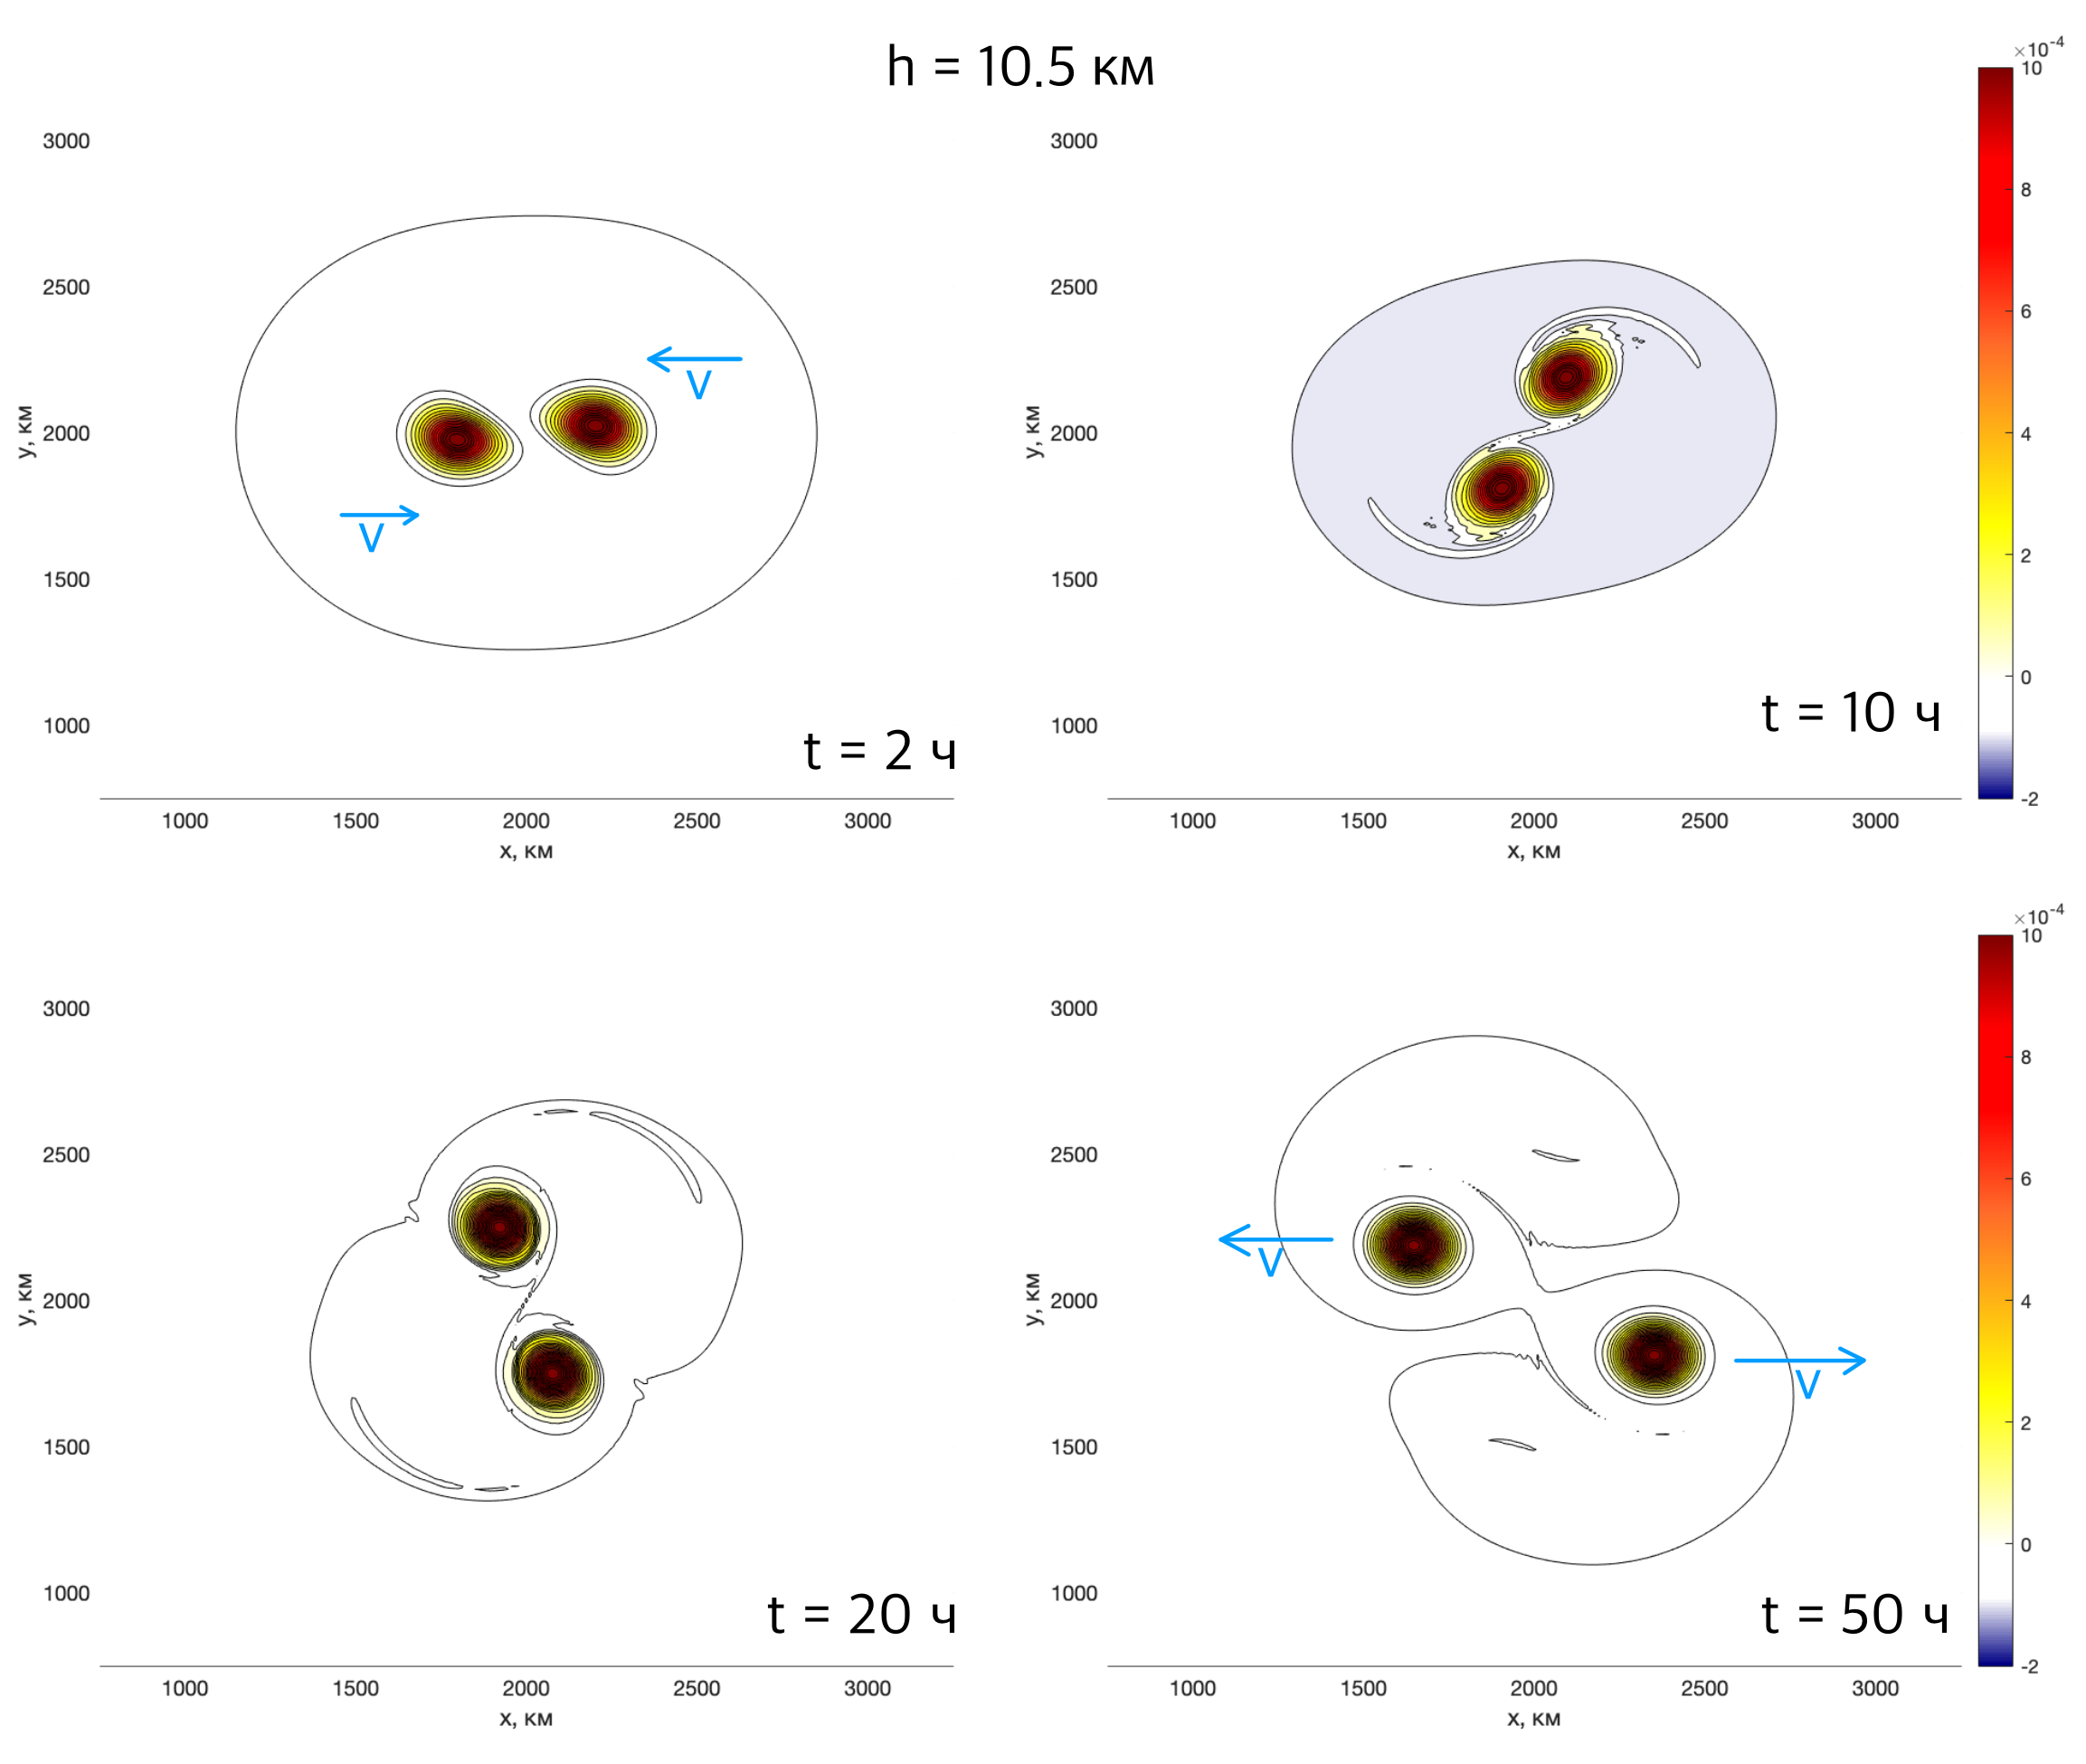
\includegraphics[width=0.7\linewidth]{./images/twocycref.png}
\caption{Поле относительной завихренности эталонного решения через 2, 10, 20, 50 часов на сетке с шагом $h = 10.5$ км}
\label{fig:mpr}
\end{figure}

\end{frame}

\begin{frame}{Взаимодействующие тропические циклоны}

\begin{figure}[h]
\centering
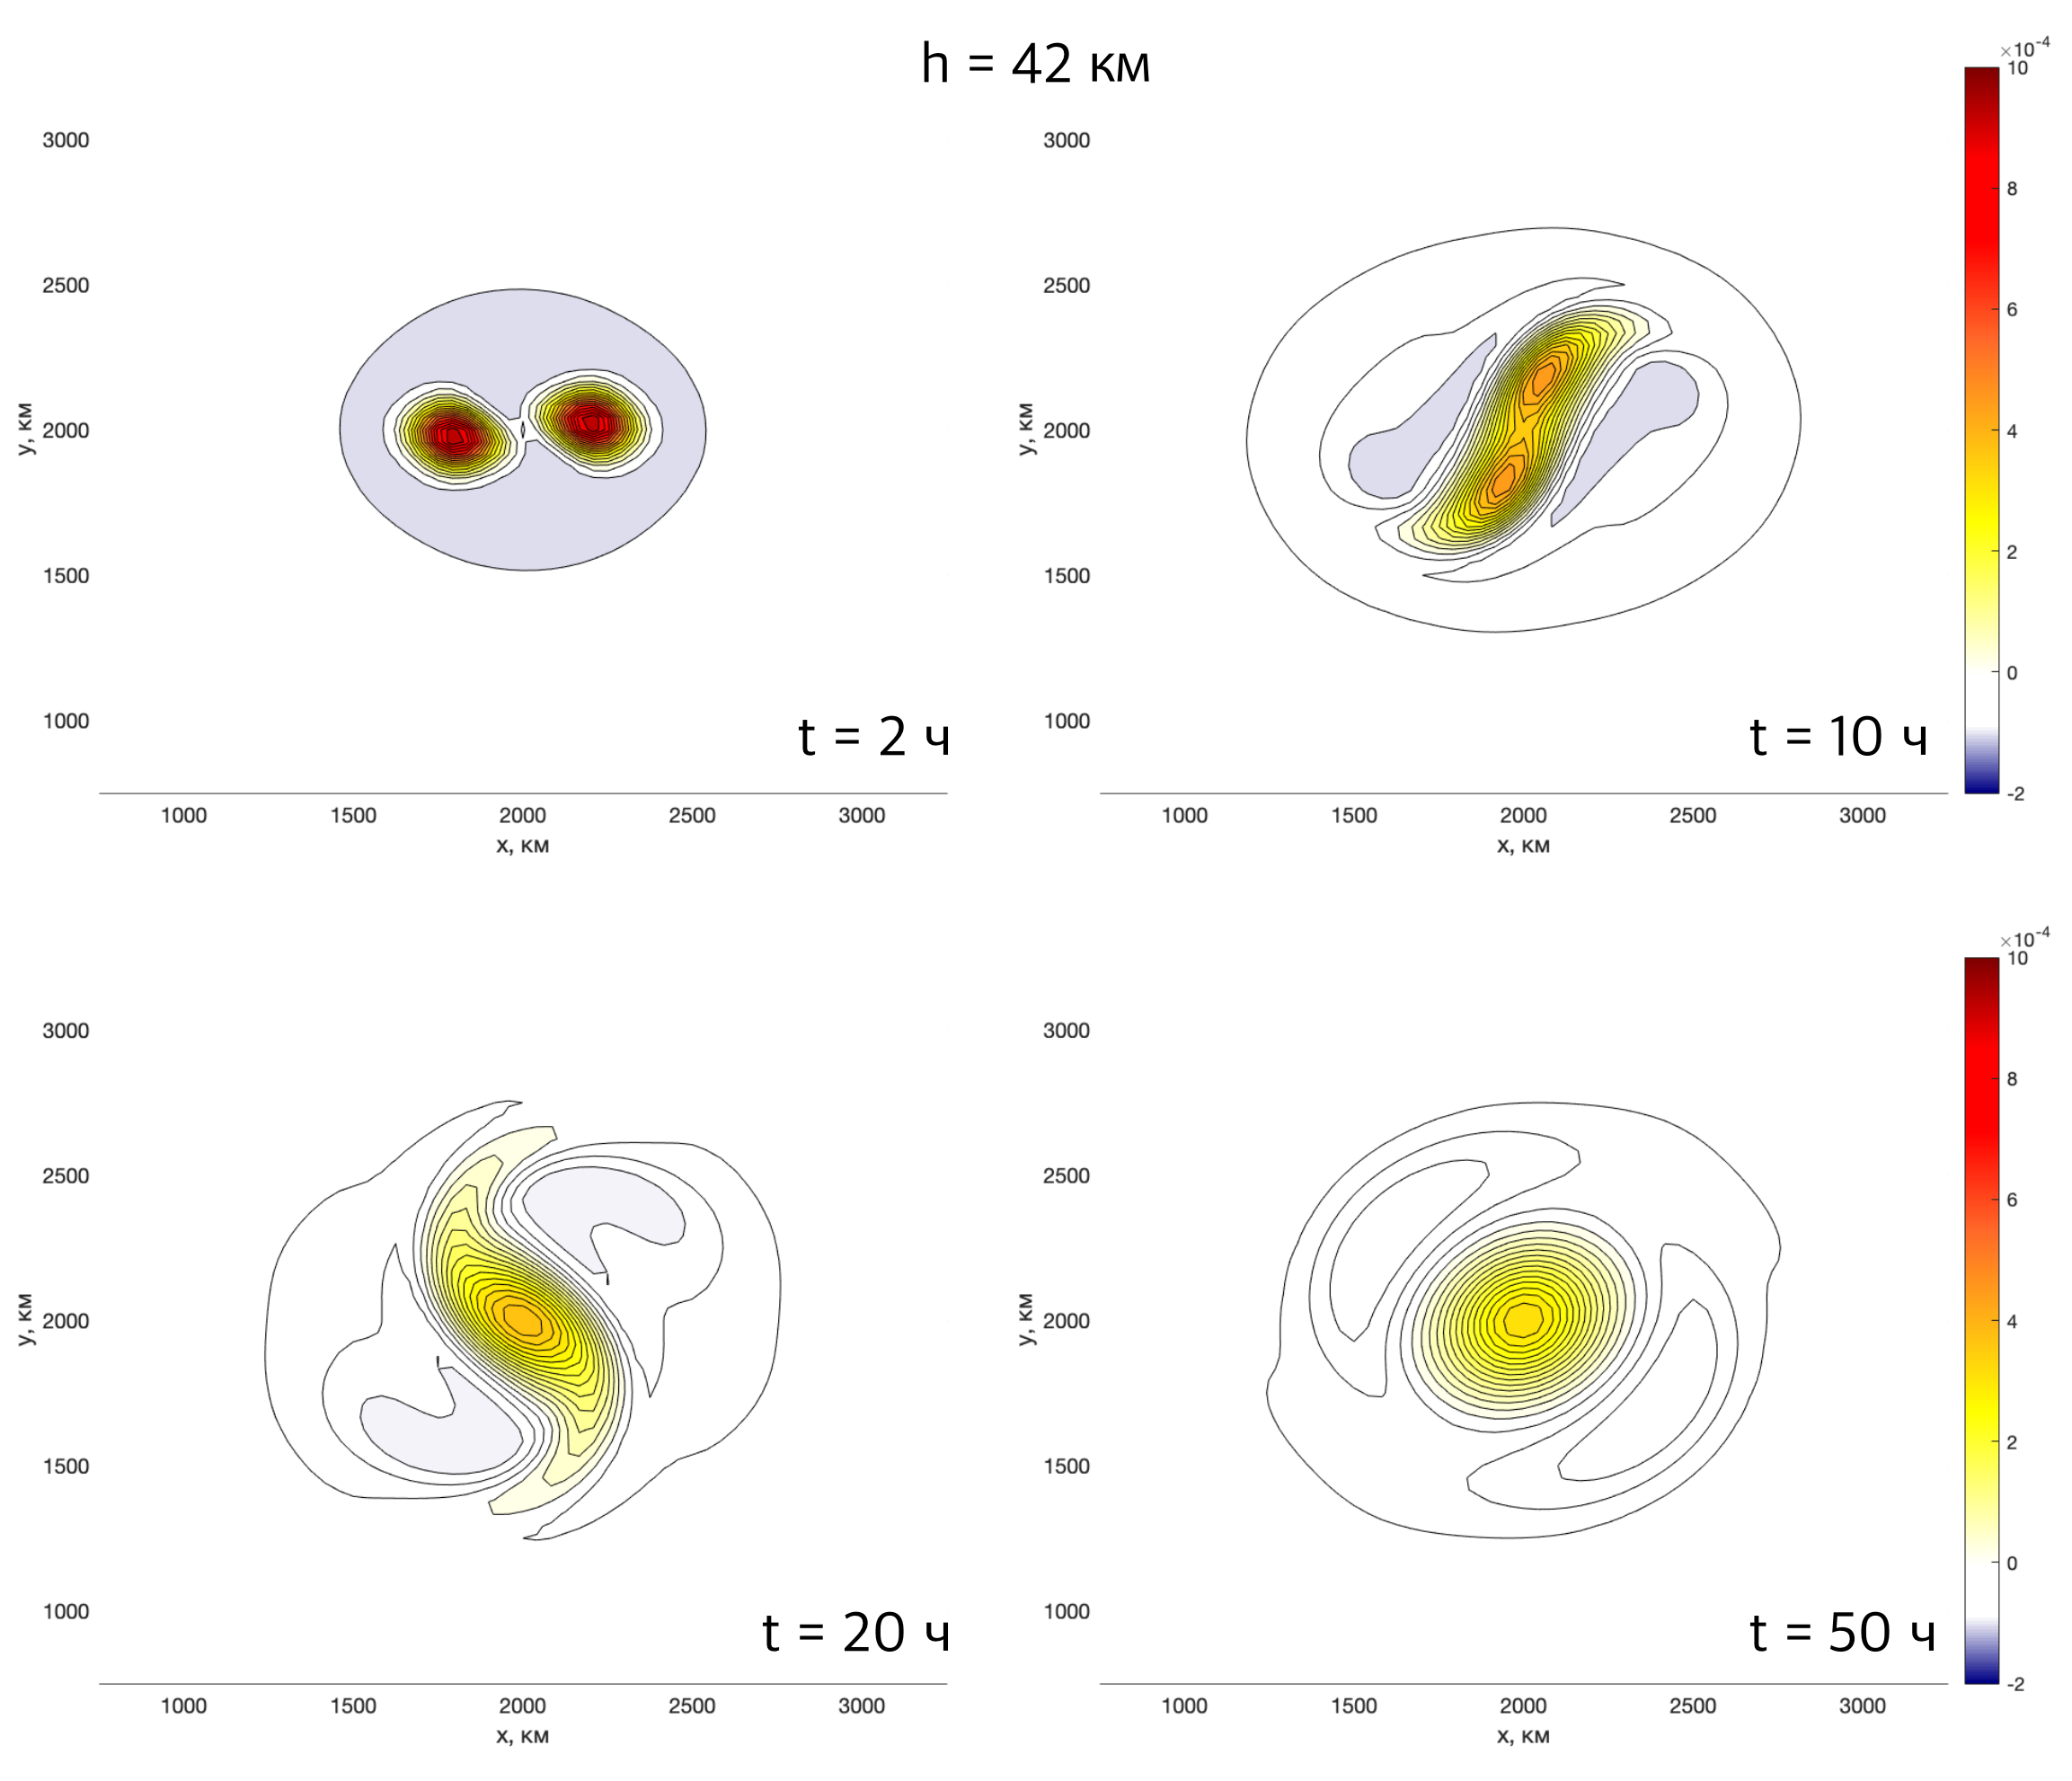
\includegraphics[width=0.7\linewidth]{./images/twocyccoarse.png}
\caption{Поле относительной завихренности решения через 2, 10, 20, 50 часов на сетке с шагом $h = 42$ км}
\label{fig:mpr}
\end{figure}

\end{frame}




\begin{frame}{Взаимодействующие тропические циклоны}

\begin{figure}[h]
\centering
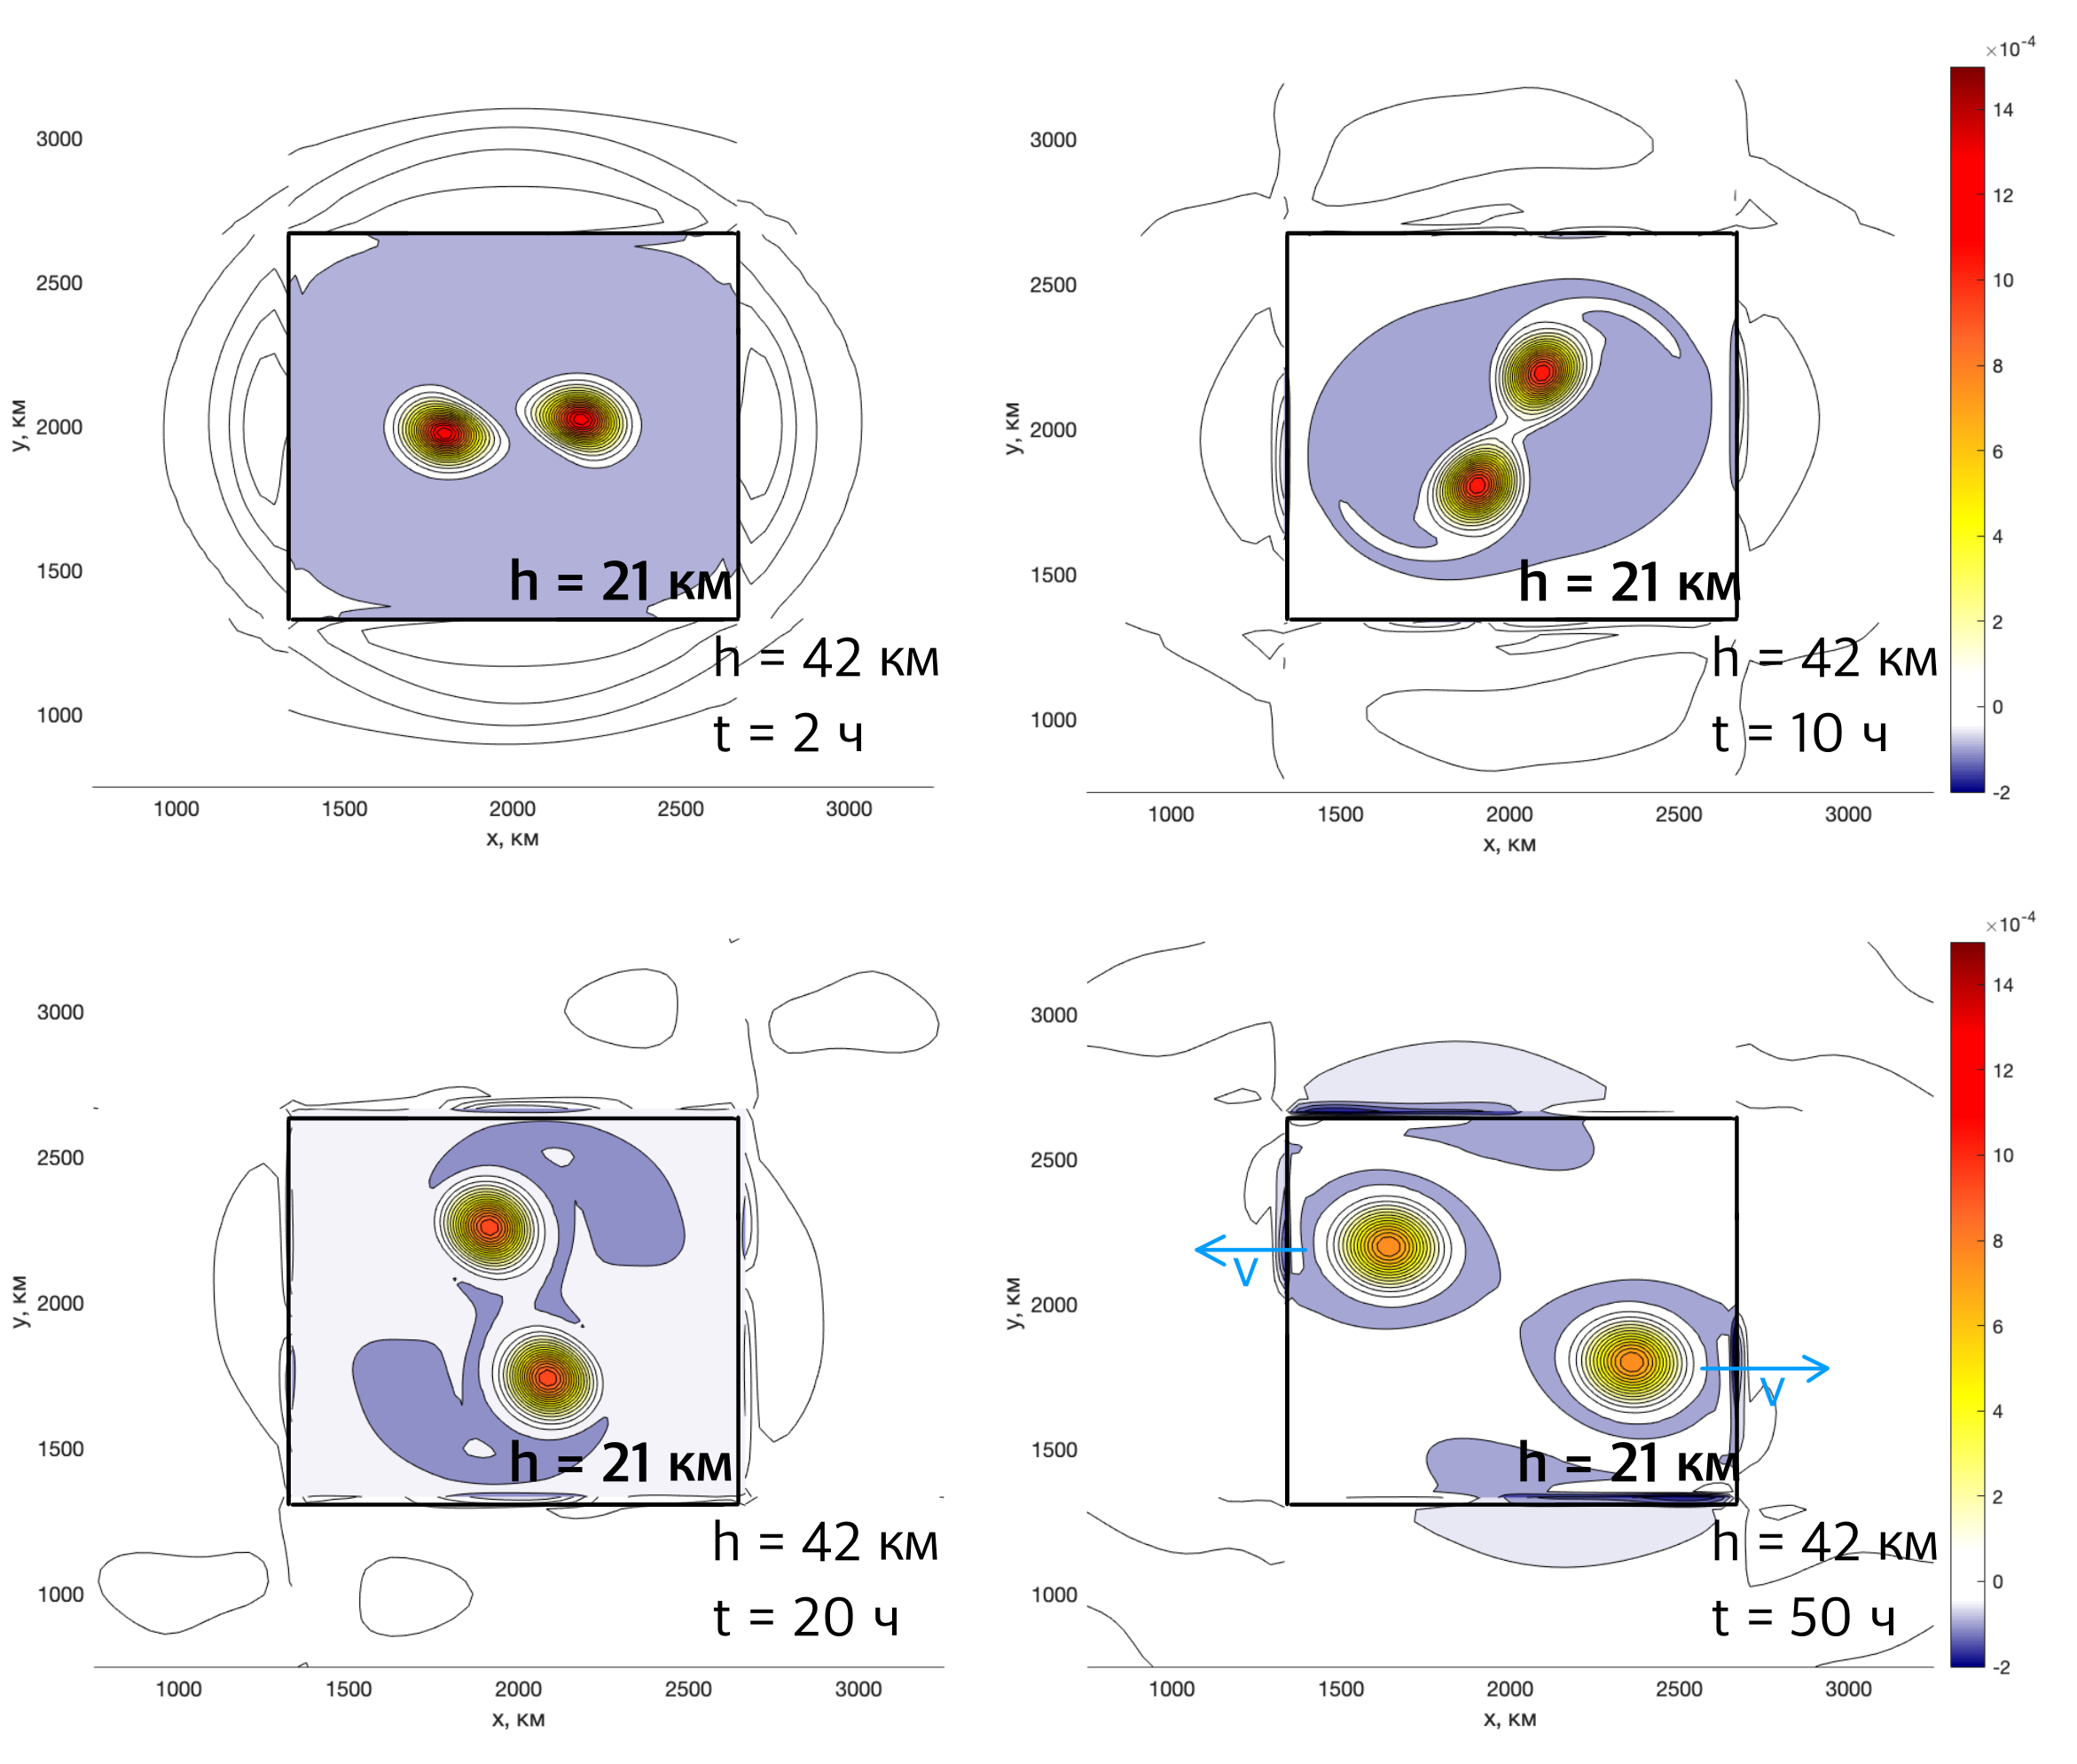
\includegraphics[width=0.7\linewidth]{./images/twocyc.png}
\caption{Поле относительной завихренности решения через 2, 10, 20, 50 часов на сетке с шагом $h = 42$ км и локальным уточнением до $h = 21$ км}
\label{fig:mpr}
\end{figure}

\end{frame}


\begin{frame}{Заключение}

Предложен подход на основе SBP-SAT метода для аппроксимации уравнений мелкой воды на сетках с локальным повышением разрешения.

\textbf{Достоинства подхода}
\begin{enumerate}
\item Сохранение массы и энергии
\item Устойчивость, доказанная теоремой
\item Высокий порядок аппроксимации
\item Локальное повышение разрешения оказывает положительное влиянение на все решение в целом
\item Удобство программной реализации
\end{enumerate}

\textbf{Недостатки подхода}
\begin{enumerate}

\item Снижение порядков аппроксимации вблизи границ блоков
\end{enumerate}

\end{frame}

\begin{frame}{Направления для дальнейших исследований}

\begin{enumerate}
\item Шаг по времени для устойчивости должен соответствовать самому мелкому разрешению
\item Реализация подхода в рамках сферической геометрии
\item Реализация подхода для трехмерных уравнений динамики атмосферы
\item Сравнение с другими методами

\end{enumerate}

\end{frame}

\begin{frame}
\center{\huge{Спасибо за внимание}}
\begin{figure}[h]
\centering
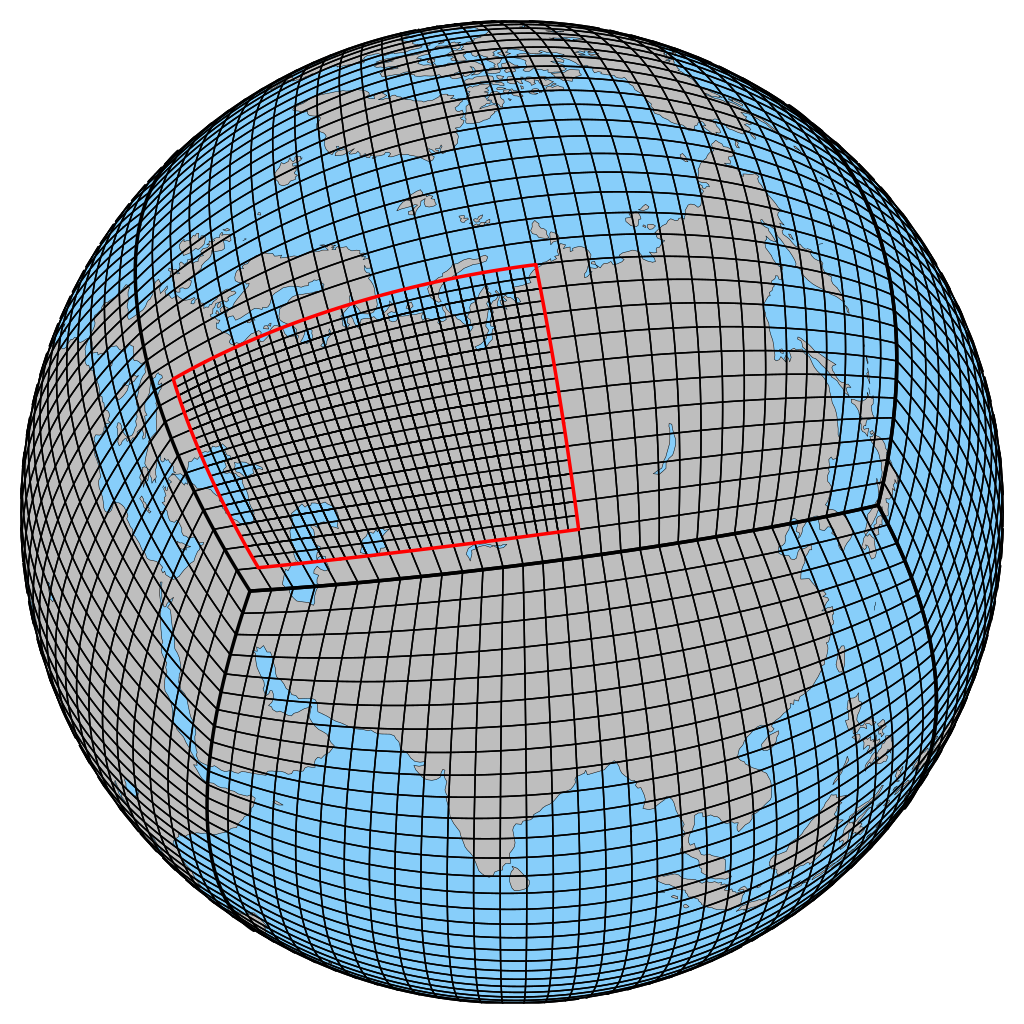
\includegraphics[width=0.4\linewidth]{./images/cubsphere.png}
\end{figure}
\end{frame}


%---------------------------------------
%       ТЕХНИЧЕСКИЕ СЛАЙДЫ
%---------------------------------------
\begin{frame}{Построение SBP-операторов}
$$\frac{\partial U}{\partial x} \approx D \textbf{u}, \ HD\textbf{u} = Q\textbf{u}$$
\begin{enumerate}
\item $H=H^T>0$, задает норму и скалярное произведение в пространстве сеточных функций  $$(\textbf{u},\textbf{v})_H=\textbf{u}^TH\textbf{v}, \ ||\textbf{u}||^2_H=\textbf{u}^TH\textbf{u}$$
\item $Q+Q^T=diag(-1,0,\ldots , 1)$
\end{enumerate}

$H,Q$ выбираются из условия удовлетворения SBP-свойству.
\end{frame}

\begin{frame}{Следствия SBP-свойства}
Если исходная задача обладает инвариантами:
$$L_1(t)=\int{U(\textbf{x},t)}d\textbf{x}, \ L_2(t)=\int{|U(\textbf{x},t)|^2}d\textbf{x}$$

Тогда дискретизованная задача сохраняет их дискртеные аналоги:
$$l_1(t) = \textbf{1}^TH\textbf{u}, \ l_2(t)=\textbf{u}^TH\textbf{u}$$

На бипериодической области выражаются дискретные аналоги законов сохранения массы и энергии.
\end{frame}

\begin{frame}{Теоремы о SBP-операторах}
\textbf{Теорема 1:} Пусть H и Q матрицы, выбранные в соответсвии с SBP-свойством. $D = H^{-1}Q$ SPB-оператор $2p$ порядка аппроксимации $\frac{d}{dx}$ внутри области. Тогда для $U\in C^{2p}(\Omega)$
$$\textbf{1}^T H \textbf{u} = \int\limits_{\Omega} {Udx} + O(h^{2p})$$

и для $V\frac{dU}{dx}\in C^{2p}(\Omega)$

$$\textbf{v}^T H D\textbf{u} = \int\limits_{\Omega}{V \frac{dU}{dx}dx} + O(h^{2p})$$
\end{frame}


\begin{frame}{Численный фильтр}
\textbf{Искусственная диссипация:}
$$\frac{\partial\psi}{\partial t}=-\kappa^2\Delta^2\psi$$

$\kappa$ - коэффициент диссипации

\begin{enumerate}
\item Дискретизация по пространству SBP-SAT подход.
\item Интегрирование про времени по явной схеме Эйлера.
\end{enumerate}

Используется для подавления пилообразных волн.
\end{frame}

\end{document}